\newpage
\chapter{Experimental Results}
\label{experiment_results}

We first present a full replication and extension of the work by \citet{radDeliberationSinglePeakednessCoherent2021a}. Then we present the simulations based on our model of meta-deliberation, as well as the results of the sensitivity analysis on both models.


\section{Replication}
We are able to fully replicate the results found by \citet{radDeliberationSinglePeakednessCoherent2021a},  in \cref{fig:rep_cyclic} we see while the bias is less than 0.73 all metric results in a-cyclic preferences. We also replicate the behavior of the KS-metric with biases in the range of 0.73-0.85, showing that it causes even some a-cyclic profiles to become cyclic. \Cref{fig:rep_transative} shows a similar graph, but instead of the number of unique preference orders present after deliberation. \citet{radDeliberationSinglePeakednessCoherent2021a} refer to these as clusters. As  we can clearly see, when bias is below 0.5, voters always agree on 1 preference order, between 0.5 and 0.73, they agree on 2 preferences for all distances. After this DP and CS both show that there is complete diversity of opinion, with all preferences being present, while KS first shows that between 0.73 and 0.85 the are 3 preference orders after deliberation, which also happen to be cyclic (we can draw this conclusion based on the fact that for this range KS introduces more cycles). Finally, after 0.85 KS behaves like DP and CS, as no voter changes their mind anymore.

\begin{figure}
	\begin{center}
		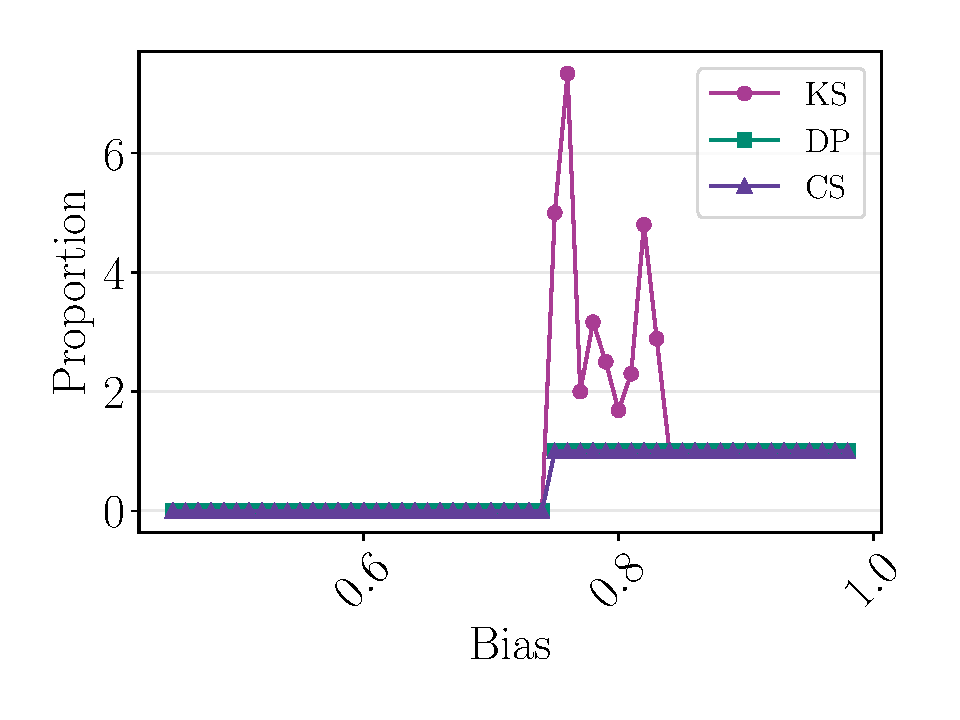
\includegraphics[width=0.65\textwidth]{Figures/cyclic_proportion_Proportion.pdf}
	\end{center}
	\caption{The proportion of cyclic profiles remaining, 0 indicating that no cyclic profiles were present after deliberation.}\label{fig:rep_cyclic}
\end{figure}

\begin{figure}
	\begin{center}
		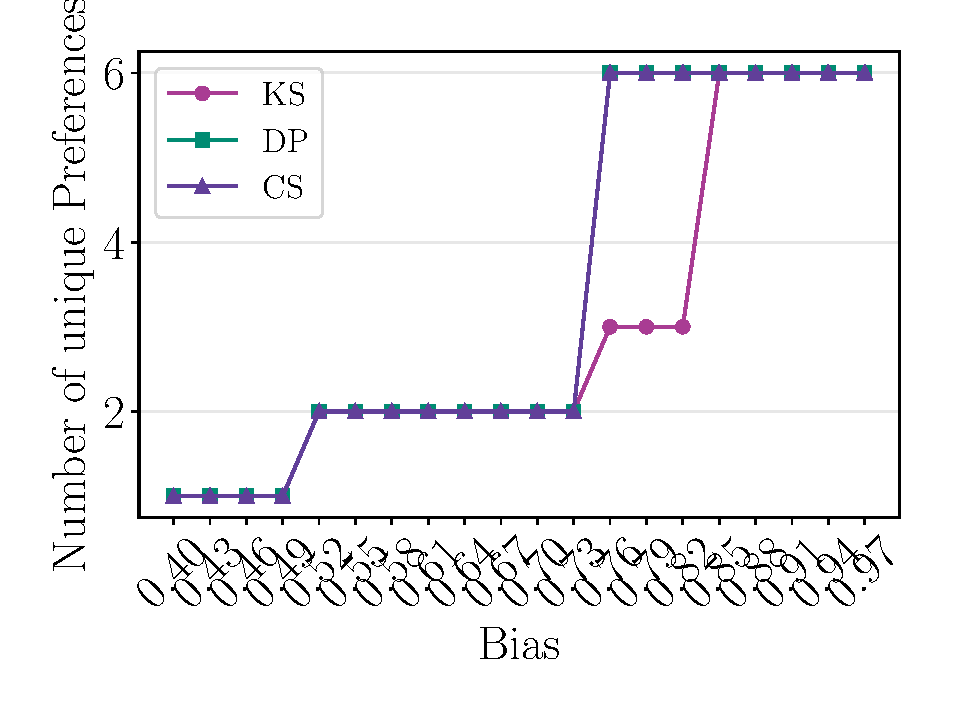
\includegraphics[width=0.65\textwidth]{Figures/Number of unique Preferences.pdf}
	\end{center}
	\caption{The proportion of intransitive profiles remaining, 0 indicating that no cyclic profiles were present after deliberation.}\label{fig:rep_transative}
\end{figure}


